\documentclass[aspectratio=169,9pt]{beamer}

% --- Typography & Core Packages ---
\usepackage[utf8]{inputenc}
\usepackage[T1]{fontenc}
\usepackage{amsmath,amssymb,amsfonts}
\usepackage{graphicx}
\usepackage{booktabs}
\usepackage{tabularx}
\usepackage{tikz}
\usetikzlibrary{shapes,arrows.meta,positioning,calc}
\usepackage{microtype}
\usepackage{multimedia}

% --- SlidePilot Native AVPlayer Compatibility Patch ---
% SlidePilot parses /Movie annotations expecting a direct string path `/Movie (file.mp4)`.
% This patch ensures the PDF annotation key is castable to String by Apple PDFKit.
\makeatletter
\renewcommand\movie[3][]{%
  \leavevmode%
  {%
    \setbox\@tempboxa=\hbox{#2}%
    \@tempdima=\wd\@tempboxa%
    \@tempdimb=\ht\@tempboxa%
    \@tempdimc=\dp\@tempboxa%
    \global\advance\mm@movie by1\relax%
    \edef\mm@label{mmdefaultlabel\the\mm@movie}%
    \def\mm@playmode{}%
    \def\mm@duration{}%
    \def\mm@start{}%
    \def\mm@poster{}%
    \def\mm@controls{}%
    \mm@autostartfalse%
    \mm@externalfalse%
    \def\mm@bw{0}%
    \setkeys{multimedia}{#1}%
    \wd\@tempboxa=\@tempdima%
    \ht\@tempboxa=\@tempdimb%
    \dp\@tempboxa=\@tempdimc%
    \beamer@pdfannot width \@tempdima height \@tempdimb depth \@tempdimc
    {
      /Subtype /Movie
      /T (\mm@label)
      /Border [0 0 \mm@bw]
      /Movie (#3)
      /A << \mm@start\space \mm@duration\space \mm@playmode\space \mm@controls\space >>
    }%
    \box\@tempboxa%
  }%
}
\makeatother

% --- Clean Minimalist Academic Theme (No bars, no rounded AI boxes) ---
\usetheme{default}
\usecolortheme{default}
\setbeamertemplate{navigation symbols}{}

% Color configuration (Crisp monochrome & high contrast)
\definecolor{darktext}{RGB}{20,24,30}
\definecolor{mutedgray}{RGB}{100,110,120}
\definecolor{lightgray}{RGB}{242,244,247}

\setbeamercolor{background canvas}{bg=white}
\setbeamercolor{normal text}{fg=darktext}
\setbeamercolor{structure}{fg=darktext}
\setbeamercolor{item}{fg=darktext}
\setbeamercolor{subitem}{fg=darktext}
\setbeamercolor{title}{fg=darktext}
\setbeamercolor{frametitle}{fg=darktext}

% Clean Frame Titles (No bars or lines)
\setbeamertemplate{frametitle}{
  \vspace{0.3em}
  {\large\bfseries\insertframetitle}
  \ifx\insertframesubtitle\@empty\else
    \\[0.1em]{\scriptsize\color{mutedgray}\insertframesubtitle}
  \fi
  \vspace{0.1em}
}

% Clean Footline (Just subtle frame number, no bars)
\setbeamertemplate{footline}{
  \hfill{\scriptsize\color{mutedgray}\insertframenumber\,/\,\inserttotalframenumber}\hspace{2.0em}\vspace{0.6em}
}

% Crisp Itemize Markers & Tight Spacing
\setbeamertemplate{itemize item}{\raisebox{0.15ex}{\tiny$\blacksquare$}}
\setbeamertemplate{itemize subitem}{\raisebox{0.15ex}{\tiny$\bullet$}}
\setbeamertemplate{itemize/enumerate body begin}{\small}
\setbeamertemplate{itemize/enumerate subbody begin}{\footnotesize}
\setlength{\leftmargini}{1.0em}
\setlength{\leftmarginii}{1.0em}

% TikZ block styles (Sharp right-angle corners, monochrome academic line-art)
\tikzset{
  sblock/.style={rectangle, draw=black, line width=0.5pt, fill=white, align=center, font=\scriptsize, inner sep=2.5pt},
  parrow/.style={-{Latex[length=1.8mm]}, thick, black},
  lbl/.style={fill=white, inner sep=1pt, font=\tiny, align=center}
}

% ==============================================================================
% PRESENTATION METADATA
% ==============================================================================
\title{Autonomous Agile Aerobatics on Micro Quadcopters}
\subtitle{Deep Reinforcement Learning and Onboard Embedded Edge Inference}
\author{Andreas Panagopoulos}
\institute{Department of Electrical and Computer Engineering\\ University of Patras, Greece}
\date{5th AI-Hub Artificial Intelligence Competition (2026)}

\begin{document}

% ------------------------------------------------------------------------------
% SLIDE 1: TITLE SLIDE
% ------------------------------------------------------------------------------
\begin{frame}[plain]
  \vspace{2.0em}
  \begin{center}
    {\LARGE\bfseries Autonomous Agile Aerobatics on Micro Quadcopters}\\[0.4em]
    {\normalsize Deep Reinforcement Learning and Onboard Embedded Edge Inference}\\[1.6em]
    
    {\normalsize\bfseries Andreas Panagopoulos}\\[0.2em]
    {\footnotesize Department of Electrical and Computer Engineering, University of Patras, Greece}\\[0.15em]
    {\scriptsize\texttt{andreas.panagopoulos@ac.upatras.gr}}\\[1.6em]
    
    {\footnotesize Technical Project Presentation -- 5th AI-Hub Competition (2026)}\\[0.2em]
    {\scriptsize Open-Source Repository: \texttt{github.com/andrupe/Quadcopter-flip}}
  \end{center}
\end{frame}

% ------------------------------------------------------------------------------
% SLIDE 2: MOTIVATION & PROBLEM STATEMENT
% ------------------------------------------------------------------------------
\begin{frame}{Motivation: An Extreme Control \& Engineering Challenge}
  \begin{columns}[onlytextwidth,T]
    \begin{column}{0.48\textwidth}
      \textbf{Why Agile Micro Quadcopters?}
      \begin{itemize}\itemsep2pt
        \item Palm-sized micro quadcopters are mechanically compliant and safe around humans, ideal for indoor confined spaces.
        \item Minimal rotational inertia enables massive angular acceleration ($>1,100^\circ/\text{s}$).
        \item \textbf{Underactuated Dynamics:} Four fixed propellers can only push upward relative to the body. To translate or stop, the entire vehicle must tilt.
        \item \textbf{The Core Value:} Performing a $360^\circ$ power flip is an extreme control benchmark, testing the absolute limits of autonomy.
      \end{itemize}
    \end{column}
    
    \begin{column}{0.48\textwidth}
      \textbf{The Primary Engineering Hurdle}
      \begin{itemize}\itemsep2pt
        \item \textbf{Maneuver Complexity:} High-speed aggressive maneuvers push quadcopter flight dynamics far beyond linear regimes, involving violent rotational rates, severe non-linear aerodynamic drag, and minimal thrust control authority during inverted flight.
        \item \textbf{Project Goal:} Execute the complete pipeline, sensing, Kalman state filtering, and neural policy inference, \textbf{100\% onboard} a single low-power microcontroller.
        \item \textbf{Thrust Headroom Reality:} Baseline 16\,mm motors have marginal thrust (T/W $\approx 1.85$), making aerobatics very hard. Upgraded motors raise mass beyond 33\,g (to $\sim 41$\,g) but provide essential control authority (T/W $\approx 2.97$).
      \end{itemize}
    \end{column}
  \end{columns}
\end{frame}

% ------------------------------------------------------------------------------
% SLIDE 3: EXPERIMENTAL SETUP: THE CRAZYFLIE 2.1
% ------------------------------------------------------------------------------
\begin{frame}{Experimental Setup: The Bitcraze Crazyflie 2.1 Platform}
  \begin{columns}[onlytextwidth,T]
    \begin{column}{0.48\textwidth}
      \textbf{Palm-Sized Micro Quadcopter}
      \begin{itemize}\itemsep2pt
        \item \textbf{Dimensions \& Mass:} 9\,cm rotor-to-rotor span; all-up mass $\sim 27-33$\,g in stock configuration.
        \item \textbf{Propulsion:} 4 brushed coreless DC motors (16\,mm baseline) with direct-drive micro propellers.
        \item \textbf{Power:} 1-cell (1S) LiPo battery (nominal 3.7\,V).
        \item \textbf{Sensors:} BMI088 IMU (1\,kHz rates) + Lighthouse deck.
      \end{itemize}
      
      \vspace{0.4em}
      \textbf{Constrained Embedded Brain}
      \begin{itemize}\itemsep2pt
        \item \textbf{STM32F405 MCU:} ARM Cortex-M4 @ 168\,MHz, 192\,KB RAM, 1024\,KB Flash.
        \item \textbf{No Linux / No Companion Coprocessor:} 100\% onboard execution without offboard assistance.
        \item \textbf{Real-Time OS:} FreeRTOS schedules radio, EKF, PWM, and neural network inference concurrently.
      \end{itemize}
    \end{column}
    
    \begin{column}{0.48\textwidth}
      \centering
      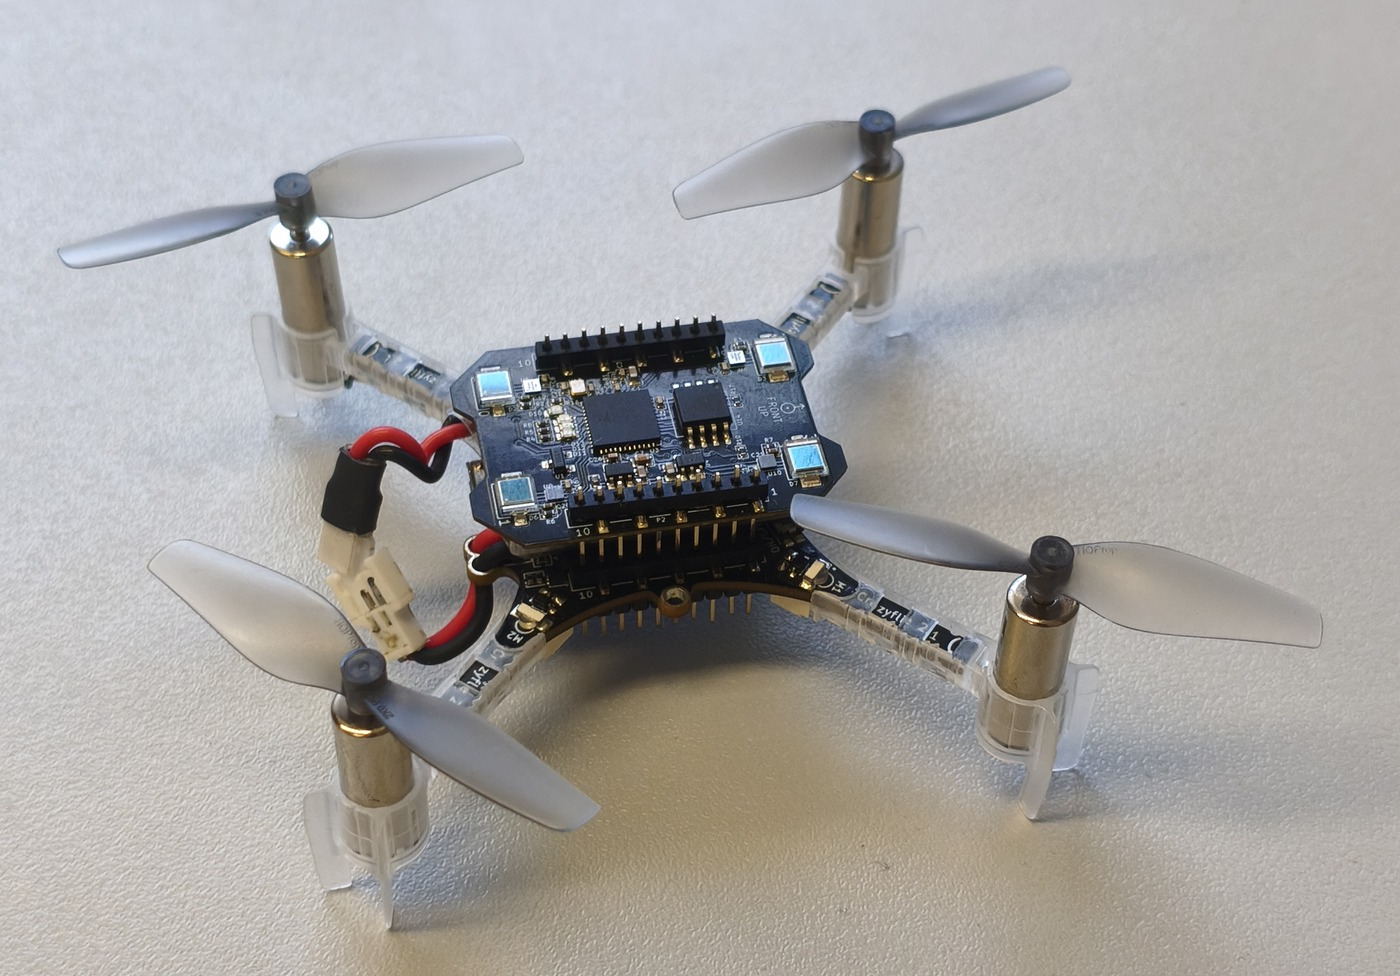
\includegraphics[width=\textwidth,height=0.60\textheight,keepaspectratio]{figures/crazyflie_hardware.jpg}\\[0.3em]
      {\scriptsize\color{mutedgray} Crazyflie 2.1 with top-mounted Lighthouse v2 deck}
    \end{column}
  \end{columns}
\end{frame}

% ------------------------------------------------------------------------------
% SLIDE 4: EXPERIMENTAL SETUP: LIGHTHOUSE OPTICAL TRACKING
% ------------------------------------------------------------------------------
\begin{frame}{Experimental Setup: Lighthouse Tracking \& The Inversion Dilemma}
  \begin{columns}[onlytextwidth,T]
    \begin{column}{0.54\textwidth}
      \textbf{How Lighthouse Optical Tracking Works}
      \begin{itemize}\itemsep2pt
        \item \textbf{External Base Stations:} Two Lighthouse v2 stations sweep rotating infrared laser beams across the flying volume.
        \item \textbf{Top-Deck Optical Receiver:} 4 photodiodes on the top deck capture pulse arrival times to solve 3D $(x, y, z)$ position onboard via Extended Kalman Filter (EKF).
      \end{itemize}
      
      \vspace{0.4em}
      \textbf{The Inversion Tracking Blackout}
      \begin{itemize}\itemsep2pt
        \item \textbf{Top-Deck Mount:} Photodiodes face up to track ceiling and wall base stations during normal upright flight.
        \item \textbf{Acrobatic Vulnerability:} During a $360^\circ$ flip, the drone rotates past $90^\circ$ tilt---the photodiodes face the floor and completely lose line of sight!
        \item \textbf{The Failure Mode:} Without optical fixes, standard EKF estimates diverge, causing standard controllers to cut throttle and crash.
      \end{itemize}
    \end{column}
    
    \begin{column}{0.42\textwidth}
      \centering
      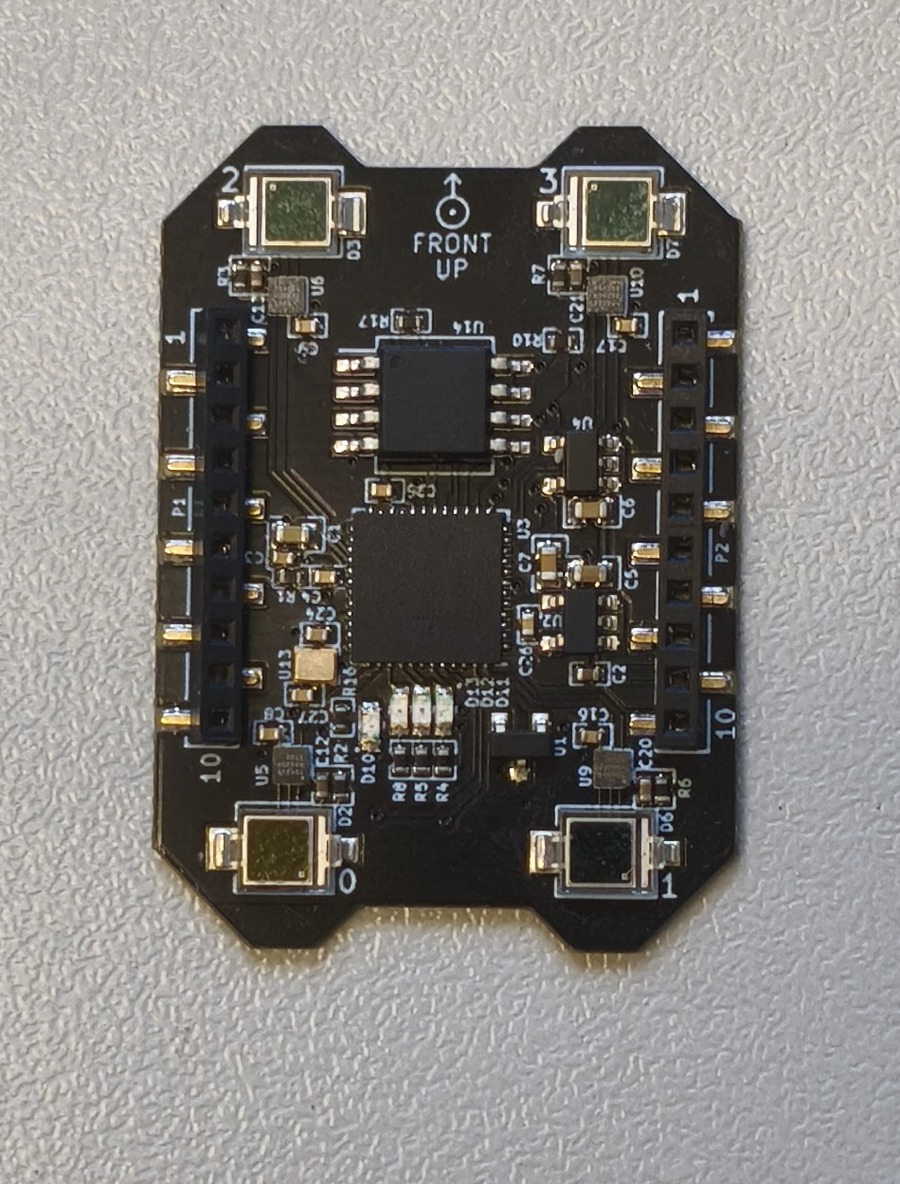
\includegraphics[width=0.74\textwidth,height=0.58\textheight,keepaspectratio]{figures/lighthouse_deck.jpg}\\[0.3em]
      {\scriptsize\color{mutedgray} Lighthouse deck with 4 corner photodiodes (0--3)}
    \end{column}
  \end{columns}
\end{frame}

% ------------------------------------------------------------------------------
% SLIDE 5: PROJECT TIMELINE & EARLY SIMULATION STRUGGLES
% ------------------------------------------------------------------------------
\begin{frame}{Project Timeline: From Simulation Struggles to Hardware}
  \begin{columns}[onlytextwidth,T]
    \begin{column}{0.48\textwidth}
      \textbf{Chronological Development Phases}
      \begin{itemize}\itemsep3pt
        \item \textbf{Phase 1: Dynamics Modeling \& Singularity Fixes}
        Rigid-body kinematics; tackling CPU throughput limits and Euler angle gimbal lock during inverted flight.
        \item \textbf{Phase 2: JAX Parallelization \& Reference Generator}
        Rewriting simulation in JAX for parallel rollouts; building an on-the-fly geometric reference generator.
        \item \textbf{Phase 3: Controller Architecture Evolution}
        Iterating from pure PPO to decoupled PPO-PID and recurrent latent history encoding.
        \item \textbf{Phase 4: Sim-to-Real Transfer \& Flight Diagnostics}
        Lab flight cage tests, analyzing radio telemetry logs, implementing firmware crash safeguards, and achieving reliable flips.
      \end{itemize}
    \end{column}
    
    \begin{column}{0.48\textwidth}
      \textbf{Early Simulation Roadblocks \& Solutions}
      \begin{itemize}\itemsep3pt
        \item \textbf{Why Not Euler Angles?}
        Standard roll, pitch, yaw ($\phi, \theta, \psi$) suffer mathematical gimbal lock at $\pm 90^\circ$ and discontinuous $180^\circ$ angle jumps during inversion. All dynamics and rewards were rebuilt using continuous \textbf{unit quaternions} $\mathbf{q} \in \mathbb{S}^3$, handling double-cover ambiguities.
        \item \textbf{From Reward Shaping to Geometric Trajectories:}
        Initially attempted pure reward shaping to coax a flip; but finding a flip from sparse rewards is extremely brittle. Transitioned to an analytic geometric controller generating smooth reference curves on the fly across multiple families (hover, waypoints, Lissajous, flips).
      \end{itemize}
    \end{column}
  \end{columns}
\end{frame}

% ------------------------------------------------------------------------------
% SLIDE 6: JAX PARALLELIZATION & TRAINING DYNAMICS
% ------------------------------------------------------------------------------
\begin{frame}{Simulation Parallelization: JAX Rewrite \& Training Dynamics}
  \begin{columns}[onlytextwidth,T]
    \begin{column}{0.48\textwidth}
      \textbf{Parallelizing Training with JAX}
      \begin{itemize}\itemsep2pt
        \item Reinforcement learning requires millions of trial-and-error interactions to discover robust control policies.
        \item Rewrote the simulation environment in \textbf{JAX} to step multiple vectorized environments simultaneously.
        \item Even on CPU, vectorization provided a \textbf{$\sim$3$\times$ to 5$\times$ speedup} over serial stepping, enabling fast hyperparameter tuning.
      \end{itemize}
      
      \vspace{0.4em}
      \textbf{Training Dynamics: Compute-Bound Progress}
      \begin{itemize}\itemsep2pt
        \item As seen on the right, episode rewards climb steadily from $\sim 160$ to $\sim 1,500$ across 30 million steps.
        \item The curve exhibits an \textbf{upward trend without plateauing}, indicating that training is \textbf{compute-bound}: additional training time would yield further performance gains.
        \item Retained tuned PPO hyperparameters: clip range $\epsilon = 0.2$, GAE $\lambda = 0.95$, and entropy regularization.
      \end{itemize}
    \end{column}
    
    \begin{column}{0.48\textwidth}
      \centering
      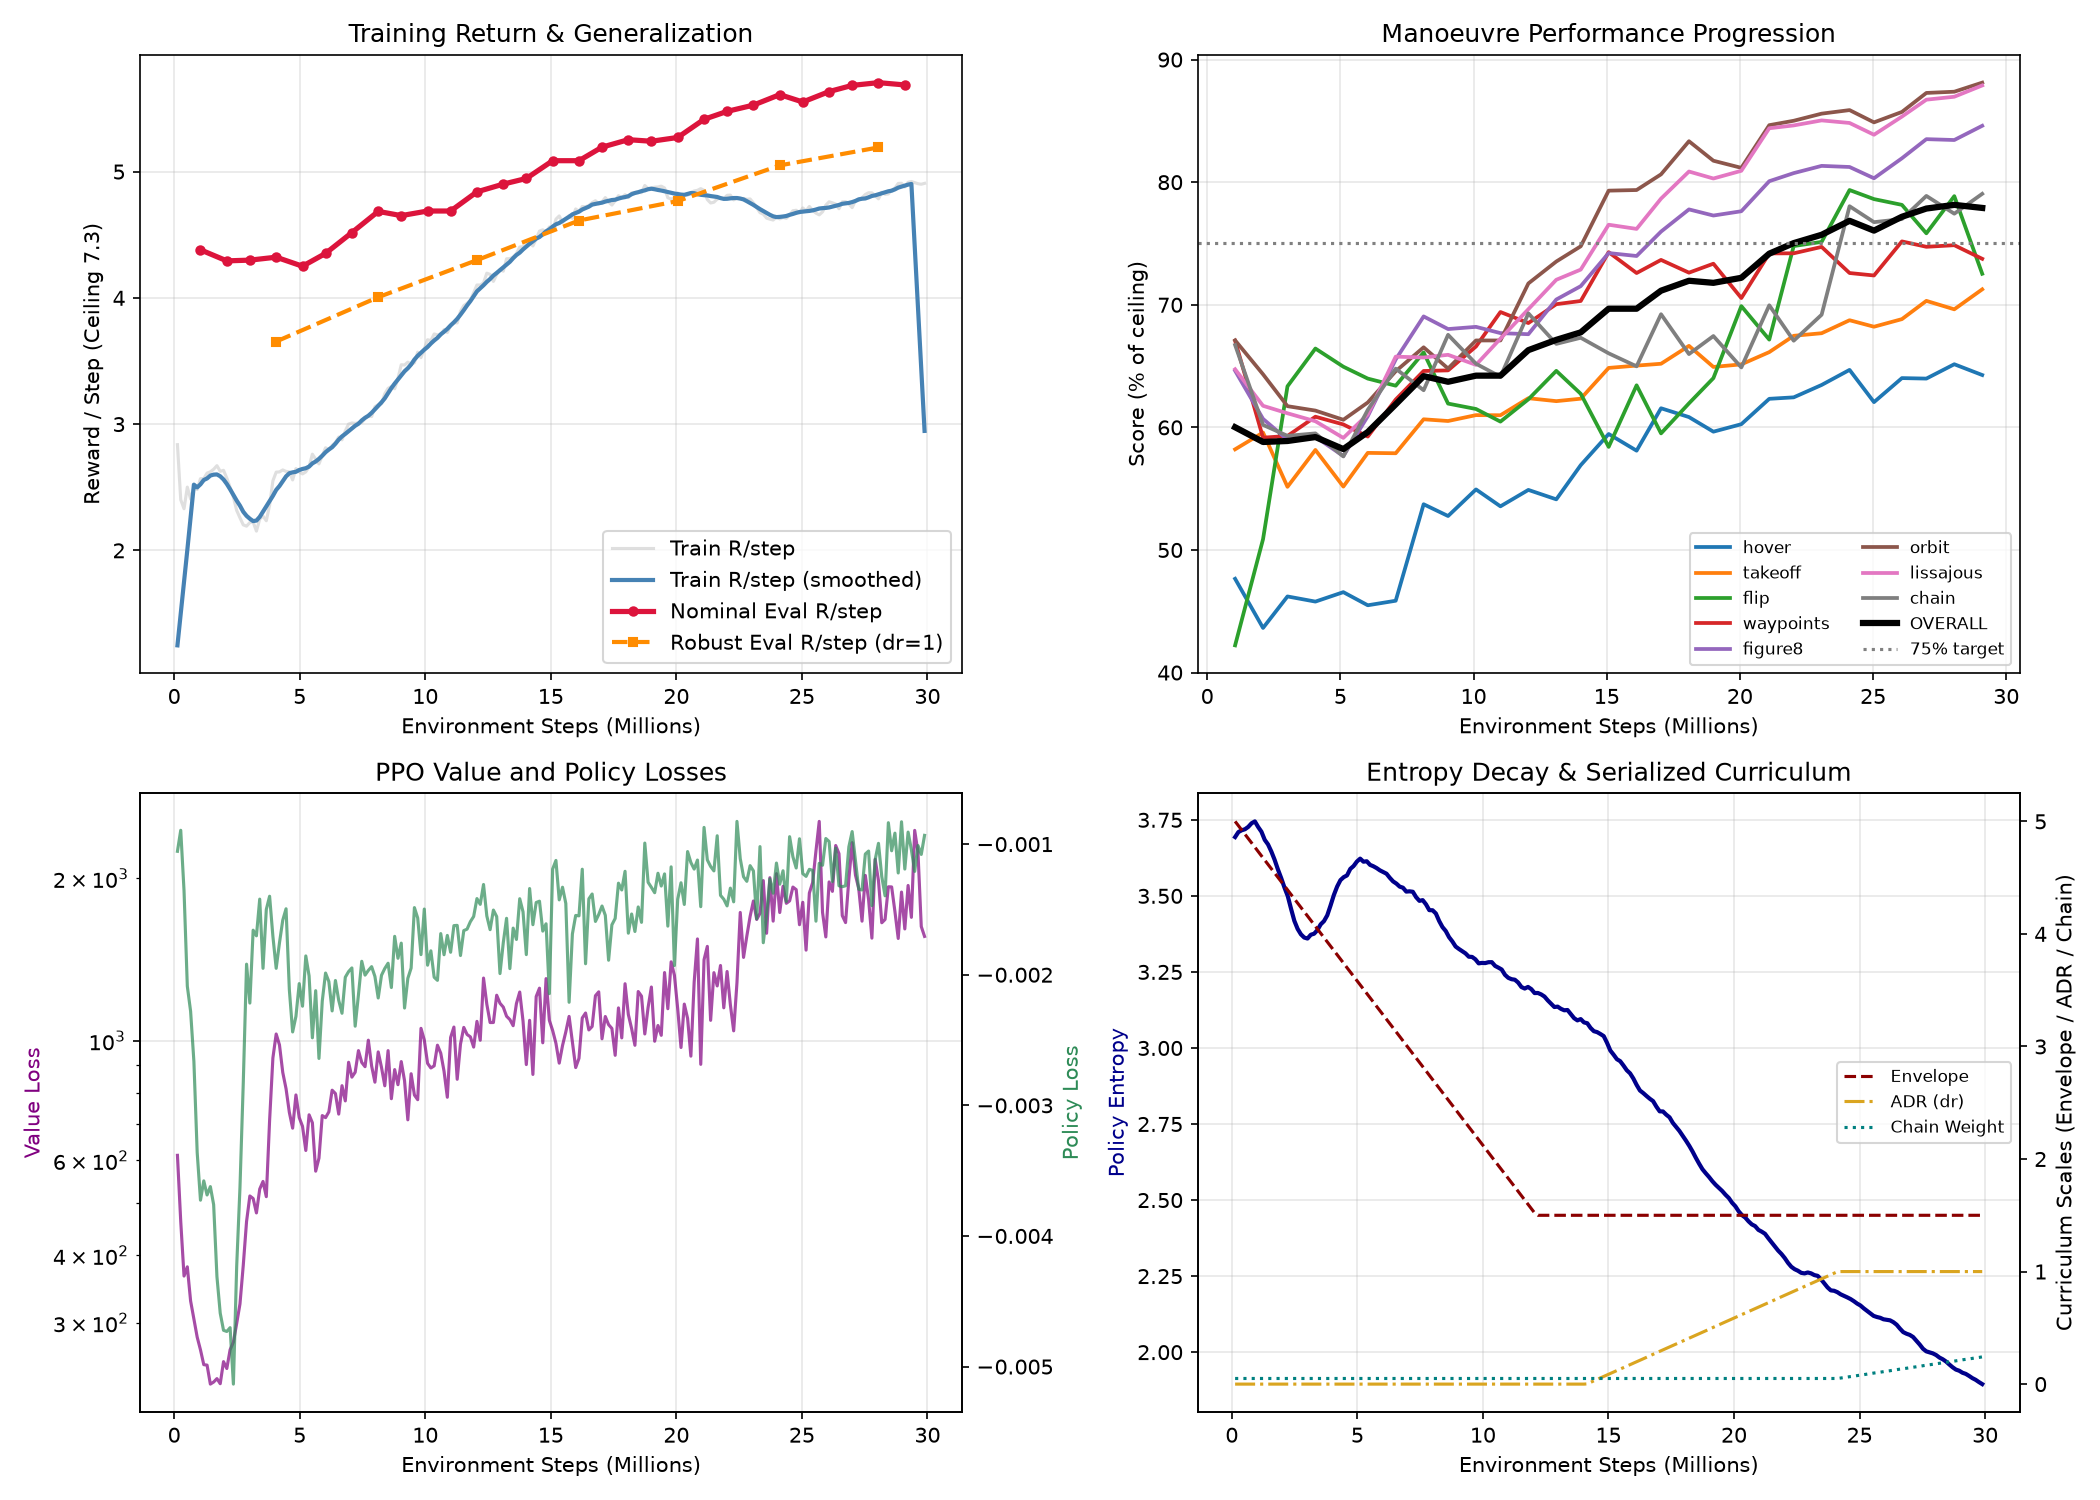
\includegraphics[width=\textwidth,height=0.55\textheight,keepaspectratio]{figures/training_curves_mjx.png}
      \vspace{0.2em}
      {\tiny\color{mutedgray} 30M-step training dynamics: upward reward progression, value convergence, and domain randomization schedule.}
    \end{column}
  \end{columns}
\end{frame}

% ------------------------------------------------------------------------------
% SLIDE 7: CONTROLLER ARCHITECTURE & DESIGN CHOICES
% ------------------------------------------------------------------------------
\begin{frame}{Controller Architecture: Actor-Critic, Asymmetry \& GRU Rationale}
  \begin{columns}[onlytextwidth,T]
    \begin{column}{0.31\textwidth}
      \textbf{Step 1: Decoupled Control}
      \begin{itemize}\itemsep2pt
        \item Pure PPO mapping directly to motor PWM caused severe motor chatter and crashes.
        \item \textbf{Decoupled Solution:} Neural policy commands 100\,Hz angular rates $\boldsymbol{\omega}_{\text{cmd}}$ and collective thrust $\tau$. Native 1\,kHz PID stabilizes motors.
      \end{itemize}
    \end{column}
    
    \begin{column}{0.33\textwidth}
      \textbf{Step 2: Asymmetric Actor-Critic}
      \begin{itemize}\itemsep2pt
        \item \textbf{Critic (Trainer):} In simulation, observes 96 privileged states (motor delay, true drag, battery sag) to reduce policy gradient variance.
        \item \textbf{Actor (Pilot):} Receives only deployable noisy sensor readings. Privileged guidance yields robust real-world generalization.
      \end{itemize}
    \end{column}
    
    \begin{column}{0.35\textwidth}
      \textbf{Step 3: Why a GRU Encoder?}
      \begin{itemize}\itemsep2pt
        \item \textbf{RNN vs.\ LSTM:} Vanilla RNNs cannot capture long-term history due to vanishing gradients, while standard LSTMs have too many gates and cannot run effectively on the STM32 MCU.
        \item \textbf{GRU Hidden State:} Holds a compact 16-D hidden state $h_t$ that captures long-term temporal dependencies recursively in-place ($O(1)$ memory).
        \item \textbf{RMA Inspiration:} Provides online adaptation to mass shifts and battery sag without retraining.
      \end{itemize}
    \end{column}
  \end{columns}
  
  \vspace{0.6em}
  \centering
  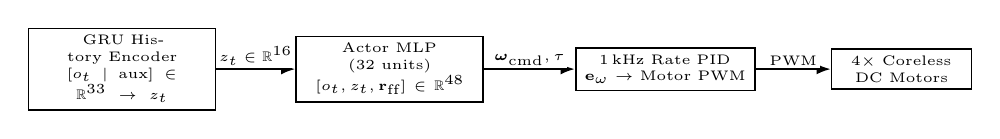
\begin{tikzpicture}[
    block/.style={rectangle, draw=black, line width=0.6pt, fill=white, align=center, font=\tiny, inner sep=2.5pt},
    parr/.style={-{Latex[length=1.8mm]}, thick, black},
    lbl/.style={fill=white, inner sep=1pt, font=\tiny, align=center}
  ]
    \node[block, text width=2.2cm] (gru) at (-5.1, 0) {GRU History Encoder\\ $[o_t \mid \text{aux}] \in \mathbb{R}^{33} \to z_t$};
    \node[block, text width=2.2cm] (act) at (-1.7, 0) {Actor MLP (32 units)\\ $[o_t, z_t, \mathbf{r}_{\text{ff}}] \in \mathbb{R}^{48}$};
    \node[block, text width=2.1cm] (pid) at (1.8, 0) {1\,kHz Rate PID\\ $\mathbf{e}_\omega \to$ Motor PWM};
    \node[block, text width=1.6cm] (mot) at (4.8, 0) {4$\times$ Coreless\\ DC Motors};
    
    \draw[parr] (gru) -- node[lbl, above] {$z_t \in \mathbb{R}^{16}$} (act);
    \draw[parr] (act) -- node[lbl, above] {$\boldsymbol{\omega}_{\text{cmd}}, \tau$} (pid);
    \draw[parr] (pid) -- node[lbl, above] {PWM} (mot);
  \end{tikzpicture}
\end{frame}

% ------------------------------------------------------------------------------
% SLIDE 8: EMBEDDED REAL-TIME DEPLOYMENT (FREERTOS)
% ------------------------------------------------------------------------------
\begin{frame}{Embedded Deployment: Deterministic Execution on FreeRTOS}
  \begin{columns}[onlytextwidth,T]
    \begin{column}{0.50\textwidth}
      \textbf{Two-Rate FreeRTOS Execution Hierarchy}
      \begin{itemize}\itemsep3pt
        \item \textbf{100\,Hz High-Level Policy Task (Every 10\,ms):}
        \begin{itemize}\itemsep1pt
          \item Acquires Lighthouse v2 tracking pose and BMI088 IMU readings.
          \item Passes data through the Estimator Plausibility Filter.
          \item Updates GRU hidden state vector and computes Actor MLP forward pass.
          \item Dispatches body rate setpoints $\boldsymbol{\omega}_{\text{cmd}}$ and collective thrust $\tau$.
        \end{itemize}
        \item \textbf{1\,kHz Low-Level Stabilizer Task (Every 1\,ms):}
        \begin{itemize}\itemsep1pt
          \item Compares rate setpoints against raw 1\,kHz gyro readings.
          \item Executes native PID feedback to generate direct motor PWM signals.
        \end{itemize}
      \end{itemize}
    \end{column}
    
    \begin{column}{0.46\textwidth}
      \textbf{Bare-Metal Embedded Engineering}
      \begin{itemize}\itemsep3pt
        \item \textbf{Strict Static Memory Allocation:}
        Neural network weights and activation buffers are compiled as static C arrays (`policy\_weights.h`, `policy\_net.c`).
        \item \textbf{Privileged Critic Discarded:}
        The large 96-D simulation critic is discarded post-training; only the compact actor MLP and GRU are compiled onto the microcontroller.
        \item \textbf{Hardware FPU Acceleration:}
        All inference computations evaluate single-precision floating-point operations directly on the ARM Cortex-M4 hardware FPU.
      \end{itemize}
    \end{column}
  \end{columns}
\end{frame}

% ------------------------------------------------------------------------------
% SLIDE 9: SIM-TO-REAL TRANSFER & THE REALITY GAP
% ------------------------------------------------------------------------------
\begin{frame}{Sim-to-Real Transfer: Overcoming the Physical Reality Gap}
  \begin{columns}[onlytextwidth,T]
    \begin{column}{0.48\textwidth}
      \textbf{The 3 Physical Roadblocks in the Lab}
      \begin{itemize}\itemsep3pt
        \item \textbf{1. Actuator Phase Lag:}
        Original 16\,mm coreless motors exhibit physical response delay ($\tau \approx 25$\,ms). At angular rates of 15--20\,rad/s, this creates a \textbf{25$^\circ$--30$^\circ$ phase lag}, triggering severe over-rotation and crashes.
        \item \textbf{2. Severe Battery Voltage Sag:}
        Demanding 100\% climb throttle causes the 1S LiPo battery to collapse from 4.1\,V down to $\sim 3.1$\,V (or 2.8\,V in back-to-back flights), reducing available thrust by $\sim 27\%$.
        \item \textbf{3. Optical Tracking Occlusion:}
        During inversion, top-mounted Lighthouse sensors lose line of sight to base stations, causing standard EKF estimators to diverge.
      \end{itemize}
    \end{column}
    
    \begin{column}{0.48\textwidth}
      \textbf{Key Physics Injected into Simulation}
      \begin{itemize}\itemsep3pt
        \item \textbf{First-Order Actuator Lag Dynamics:}
        $\dot{\omega}_{M,i} = \frac{1}{\tau} (\omega_{M,i}^{\text{cmd}} - \omega_{M,i})$ with randomized time constant $\tau \in [18, 35]$\,ms.
        \item \textbf{Coupled Battery Voltage Sag Modeling:}
        Modeled dynamic voltage sag as a function of instantaneous throttle draw and battery state-of-charge.
        \item \textbf{Aerodynamic Drag \& Precession:}
        Coupled non-linear drag tensors and rotor gyroscopic torques during high-rate pitch maneuvers.
        \item \textbf{Domain Randomization:}
        Perturbed vehicle mass, inertia tensors, motor thrust coefficients, and sensor noise variances.
      \end{itemize}
    \end{column}
  \end{columns}
\end{frame}

% ------------------------------------------------------------------------------
% SLIDE 10: FIRMWARE SAFEGUARDS & MOTOR TRANSFER ADAPTATION
% ------------------------------------------------------------------------------
\begin{frame}{Firmware Safeguards \& Motor Transfer Adaptation}
  \begin{columns}[onlytextwidth,T]
    \begin{column}{0.48\textwidth}
      \textbf{Firmware Precautions \& Safeguards}
      \begin{itemize}\itemsep2pt
        \item \textbf{Crash Precautions:} Took practical firmware precautions to protect the drone and prevent occasional crashes during aggressive maneuvers.
        \item \textbf{Estimator Plausibility Filter:}
        Pre-processing filter after the Kalman estimator that rejects unphysical jumps (e.g.\ teleporting states). When optical tracking drops during inversion, it freezes estimates at the last valid reading and temporarily suspends false altitude aborts.
        \item \textbf{Debounced Ground Failsafe:}
        Smoothly ramps thrust to zero over 1.2\,s in self-leveling attitude mode instead of cutting props abruptly.
        \item \textbf{Iterative Lab Loop:}
        Flying in the safety cage, analyzing 100\,Hz telemetry logs, and updating simulation parameters.
      \end{itemize}
    \end{column}
    
    \begin{column}{0.48\textwidth}
      \textbf{Motor Transfer Adaptation (RMA)}
      \begin{itemize}\itemsep2pt
        \item \textbf{Plant Upgrade:} Installed upgraded 20\,mm motors (right) vs.\ 16\,mm baseline (left), raising peak thrust to 1.19\,N (mass: 41\,g, T/W: 2.97).
        \item \textbf{Motor Transfer Adaptation:} Completed flips \textbf{without retraining}! The GRU latent vector $z_t$ absorbed mass and thrust changes online.
      \end{itemize}
      
      \vspace{0.2em}
      \centering
      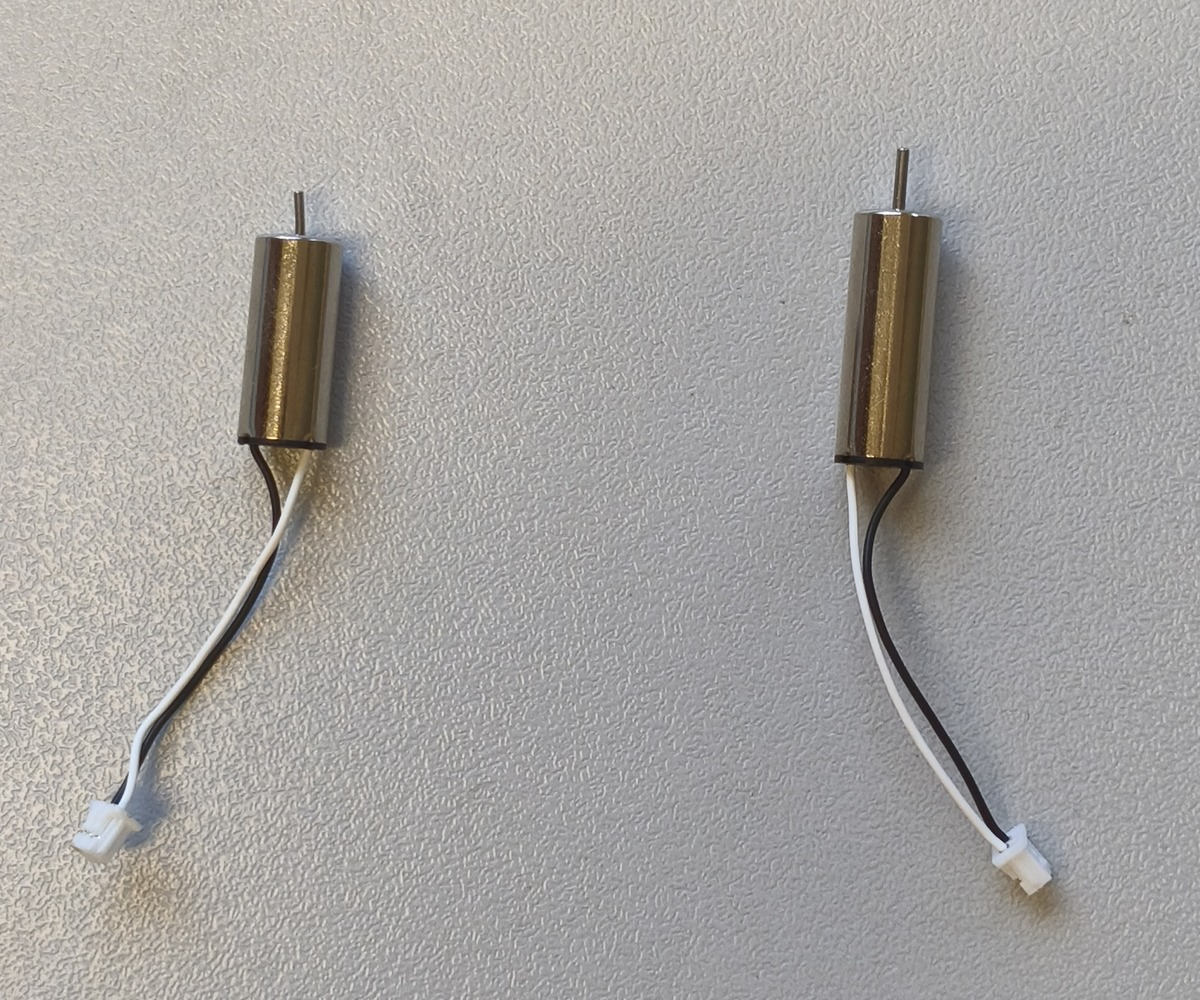
\includegraphics[width=0.70\textwidth,height=0.34\textheight,keepaspectratio]{figures/motors_16mm_vs_20mm.jpg}\\[0.2em]
      {\scriptsize\color{mutedgray} Motor upgrade: 16\,mm (left) vs.\ 20\,mm (right)}
    \end{column}
  \end{columns}
\end{frame}

% ------------------------------------------------------------------------------
% SLIDE 11: EXPERIMENTAL FLIGHT RESULTS (REAL FLIGHT LOG DATA)
% ------------------------------------------------------------------------------
\begin{frame}{Experimental Flight Results: Hardware Flight Log Telemetry}
  \begin{columns}[onlytextwidth,T]
    \begin{column}{0.48\textwidth}
      \textbf{Measured Hardware Maneuver Phases (Flight \#6)}
      \begin{itemize}\itemsep3pt
        \item \textbf{Phase 1: Climb Pop (t = 7.92 -- 8.65\,s)}
        Policy commands saturated thrust; vehicle climbs from 1.22\,m to peak \textbf{$z = 1.82$\,m} (+0.60\,m pop clearance). Battery voltage sags to 3.33\,V.
        \item \textbf{Phase 2: Inverted Ballistic Coast (t = 8.65 -- 8.94\,s)}
        Thrust reduced; rapid pitch rotation reaches \textbf{158$^\circ$ inversion}. Optical reception collapses to 0 packets; the Plausibility Gate holds state continuity.
        \item \textbf{Phase 3: Catch \& Upright Recovery (t = 8.94 -- 9.46\,s)}
        Counter-torque halts rotation, thrust ramps to arrest descent, recovering tilt to \textbf{16$^\circ$} and touching down upright without tumbling (`sup\_bits` remained 542).
      \end{itemize}
    \end{column}
    
    \begin{column}{0.48\textwidth}
      \centering
      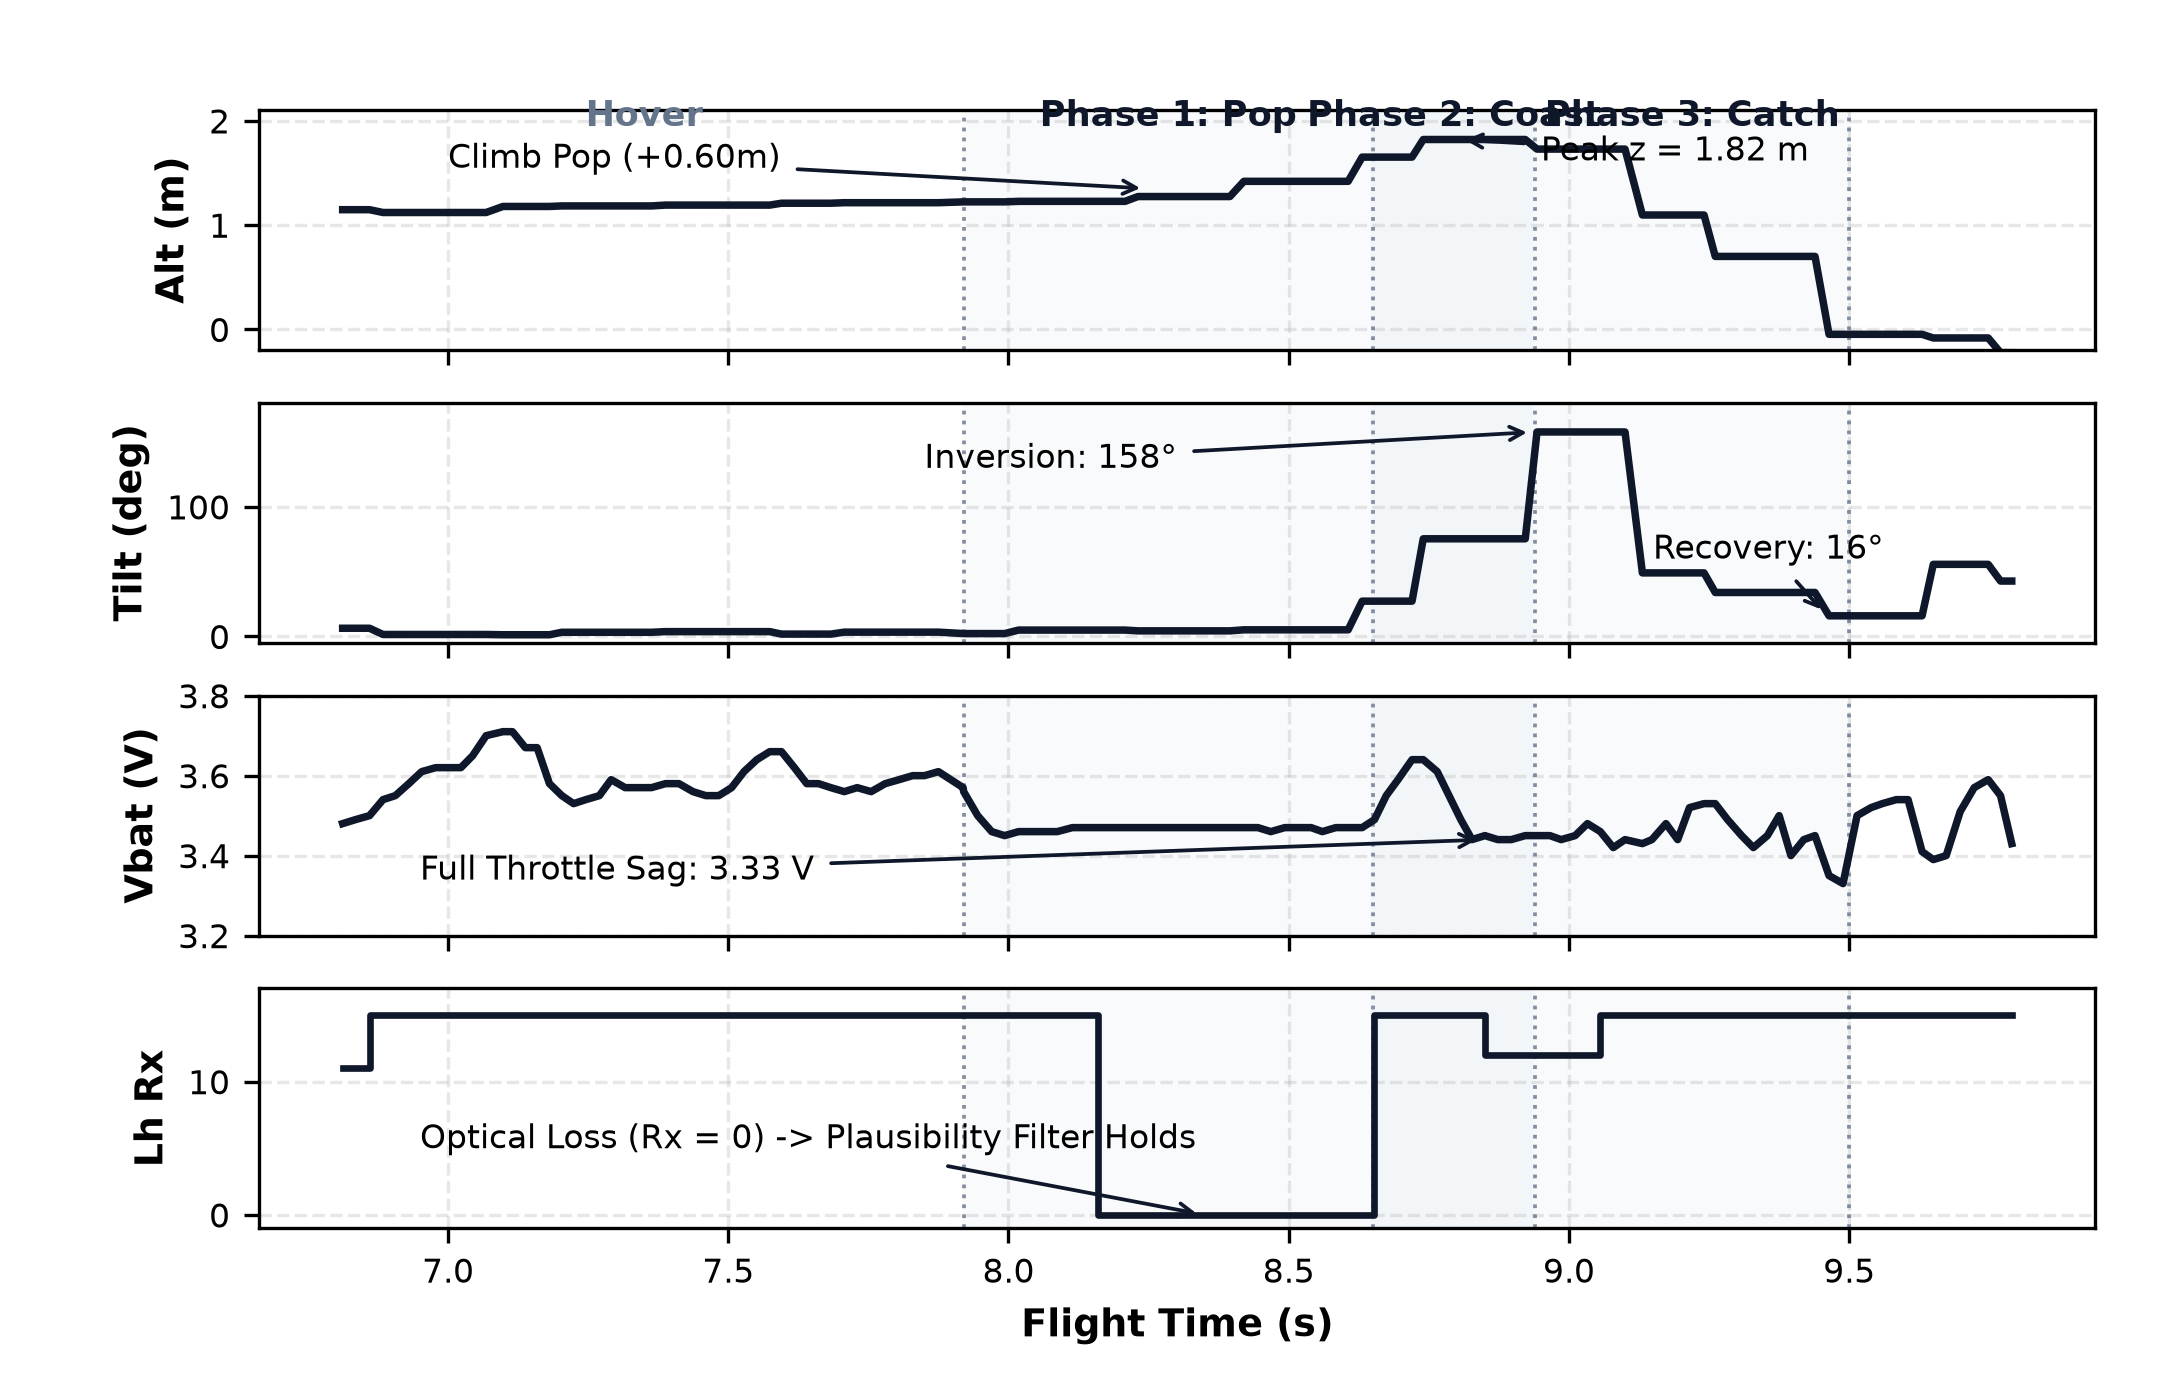
\includegraphics[width=\textwidth,height=0.55\textheight,keepaspectratio]{figures/real_flight_telemetry.png}
      \vspace{0.2em}
      {\tiny\color{mutedgray} Real 100\,Hz hardware flight log (Flight \#6): climb pop ($z=1.82$\,m), $158^\circ$ inversion tilt, battery voltage sag, and optical occlusion resilience.}
    \end{column}
  \end{columns}
\end{frame}

% ------------------------------------------------------------------------------
% SLIDE 12: EMPIRICAL FLIGHT DEMONSTRATION (SIMULATION VS. REAL FLIGHT)
% ------------------------------------------------------------------------------
\begin{frame}{Empirical Flight Demonstration: Simulation vs.\ Real Flip}
  \begin{columns}[onlytextwidth,T]
    % Simulation Video Column
    \begin{column}{0.48\textwidth}
      \centering
      {\small\bfseries MuJoCo MJX Physics Simulation}\\[0.3em]
      \movie[width=\linewidth,height=0.5625\linewidth,poster,showcontrols]{%
        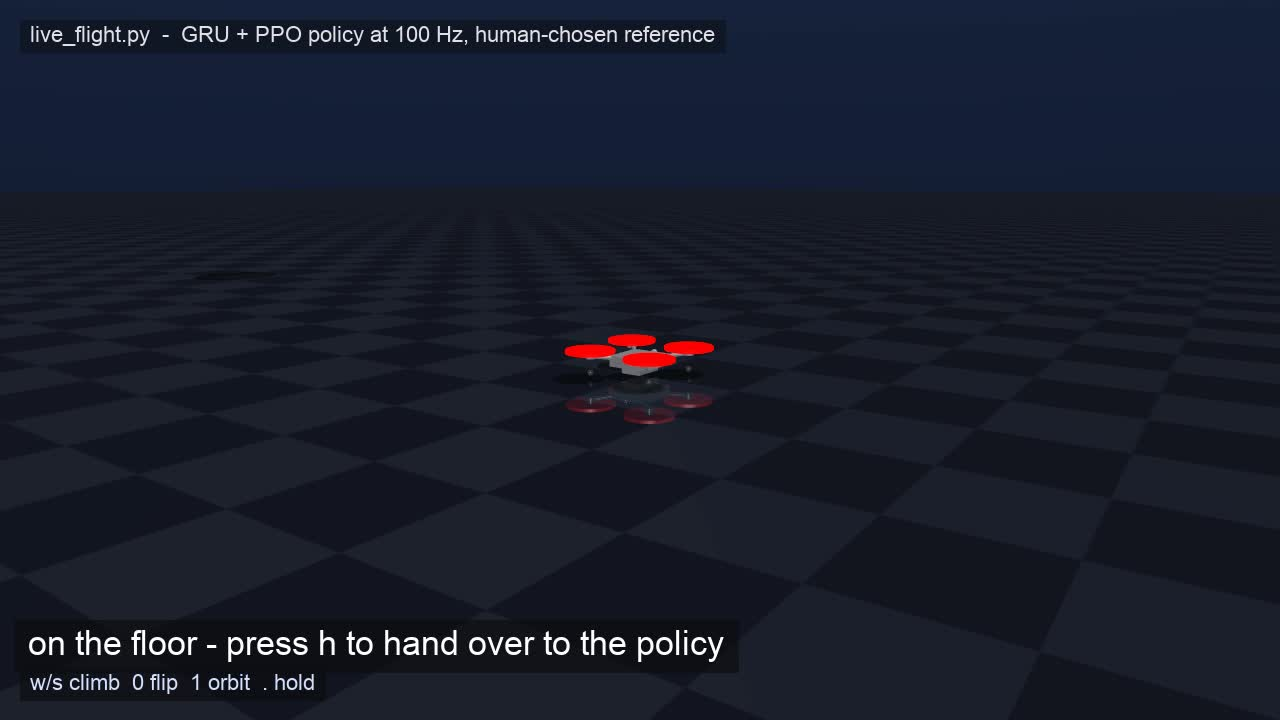
\includegraphics[width=\linewidth,height=0.5625\linewidth]{figures/poster_sim_flip.jpg}%
      }{videos/sim_vid.mp4}\\[0.4em]
      {\scriptsize\color{mutedgray} Continuous pitch flips in vectorized MJX physics environment}
    \end{column}

    % Real Flight Video Column
    \begin{column}{0.48\textwidth}
      \centering
      {\small\bfseries Physical Hardware Flight}\\[0.3em]
      \movie[width=\linewidth,height=0.5625\linewidth,poster,showcontrols]{%
        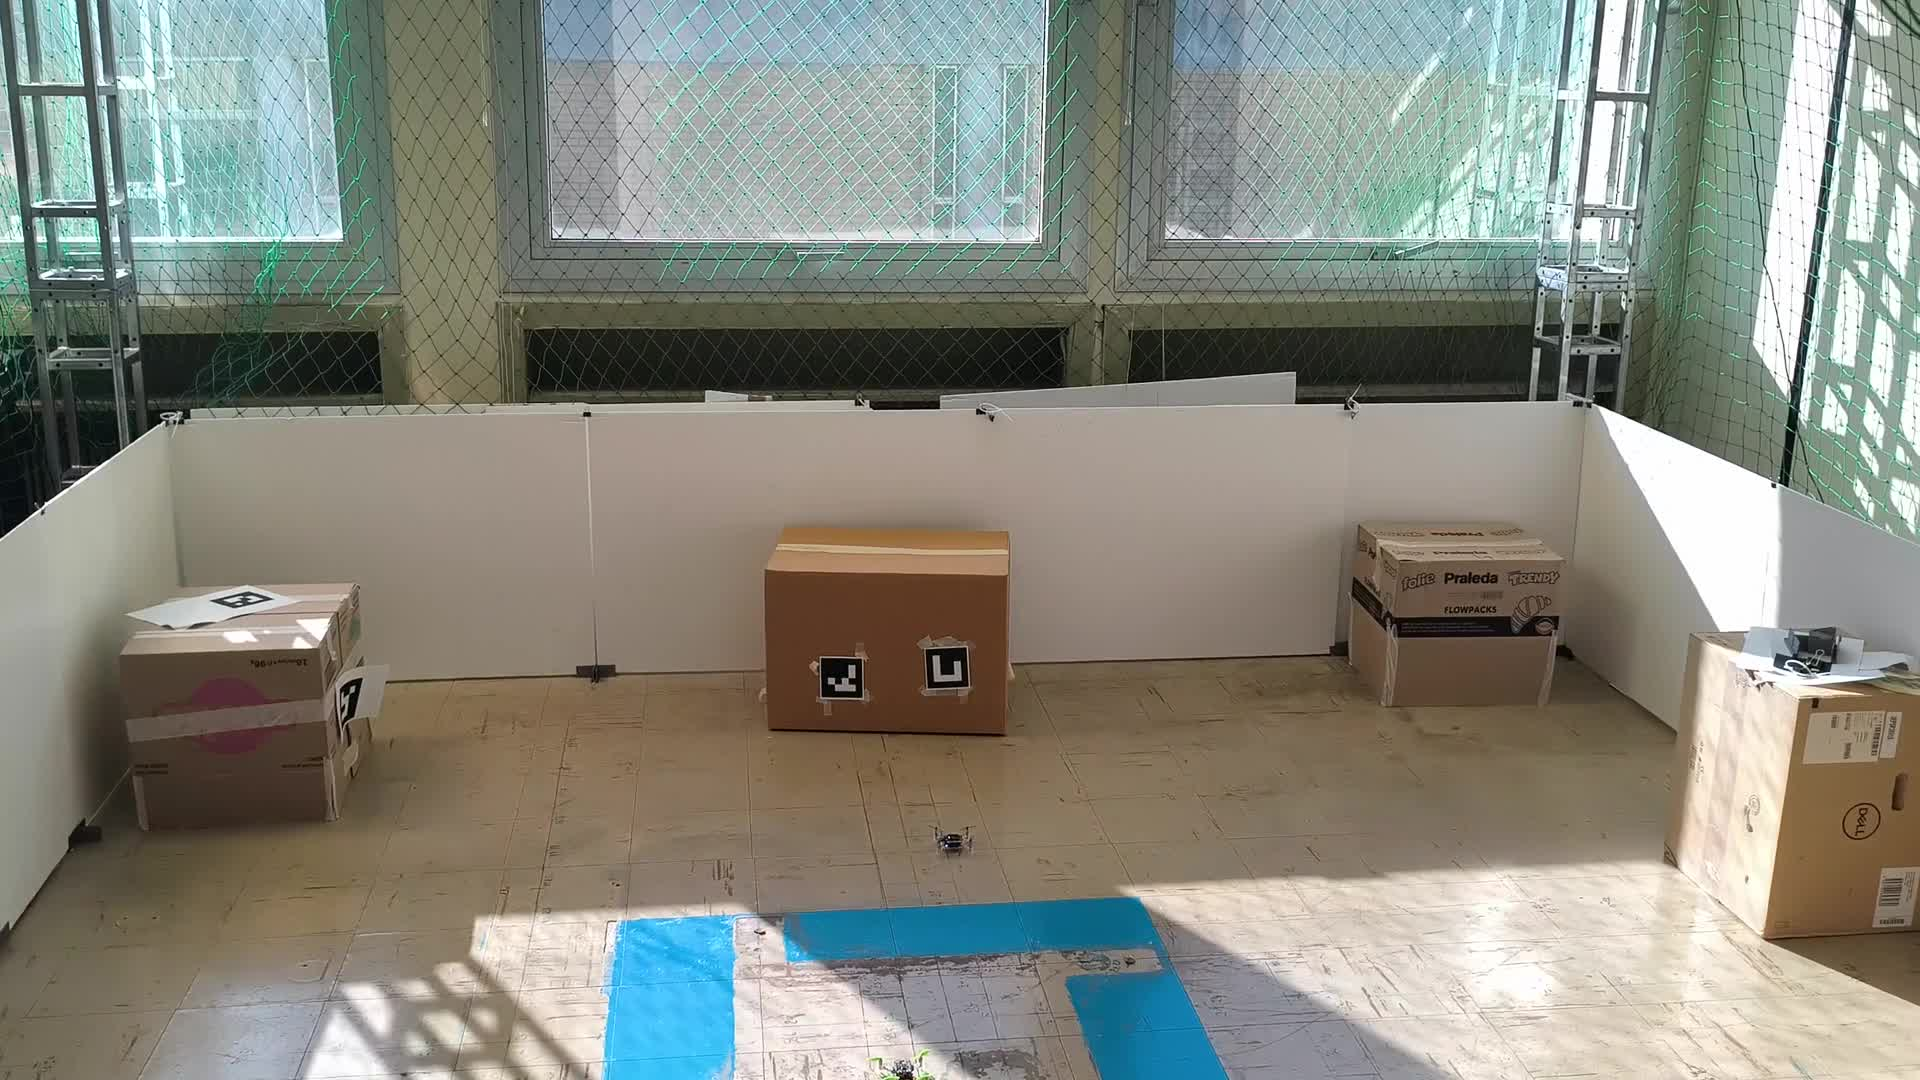
\includegraphics[width=\linewidth,height=0.5625\linewidth]{figures/poster_real_flip.jpg}%
      }{videos/real_vid.mp4}\\[0.4em]
      {\scriptsize\color{mutedgray} Autonomous onboard $360^\circ$ power flip \& upright catch}
    \end{column}
  \end{columns}

  \vspace{0.6em}
  \centering
  {\scriptsize\color{mutedgray} Click on either video to play inline in \textbf{SlidePilot}. (In \textbf{Apple Preview}, \href{run:videos/real_vid.mp4}{\underline{click here to open in QuickTime}}).}
\end{frame}

% ------------------------------------------------------------------------------
% SLIDE 13: FUTURE EXTENSIONS & TECHNICAL USE CASES
% ------------------------------------------------------------------------------
\begin{frame}{Looking Ahead: Technical Improvements \& Practical Use Cases}
  \begin{columns}[onlytextwidth,T]
    \begin{column}{0.48\textwidth}
      \textbf{Future Technical Extensions}
      \begin{itemize}\itemsep3pt
        \item \textbf{Onboard Visual-Inertial Odometry (VIO):}
        Integrating ultra-light optical flow camera sensors to eliminate dependency on external Lighthouse tracking stations entirely.
        \item \textbf{Arbitrary Initial Condition Tumble Recovery:}
        Expanding the training curriculum to initialize episodes from arbitrary tumbling states, enabling recovery from mid-air collisions.
        \item \textbf{Scaling Training Compute:}
        Leveraging the observed upward compute-bound training dynamics by scaling training steps to further refine trajectory tracking accuracy.
      \end{itemize}
    \end{column}
    
    \begin{column}{0.48\textwidth}
      \textbf{Realistic Real-World Applications}
      \begin{itemize}\itemsep3pt
        \item \textbf{Agile Micro-Aerial Robotics:}
        Enabling autonomous micro quadcopters to navigate highly dynamic, cluttered environments with extreme agility.
        \item \textbf{Confined Industrial Inspection:}
        Navigating narrow conduits, complex pipes, and industrial machinery where physical access is strictly limited.
        \item \textbf{Extreme Maneuver Autonomy:}
        Establishing robust baseline neural controllers for aggressive aerobatic trajectories in restricted indoor flight envelopes.
      \end{itemize}
    \end{column}
  \end{columns}
\end{frame}

% ------------------------------------------------------------------------------
% SLIDE 14: SUMMARY & CONCLUSION
% ------------------------------------------------------------------------------
\begin{frame}{Project Summary: Autonomous Edge AI Control}
  \begin{columns}[onlytextwidth,T]
    \begin{column}{0.54\textwidth}
      \textbf{Key Project Takeaways}
      \begin{itemize}\itemsep3pt
        \item \textbf{Autonomous Onboard Aerobatics:} Proved that deep reinforcement learning can control extreme $360^\circ$ flips entirely onboard an ARM Cortex-M4 microcontroller without offboard assistance.
        \item \textbf{JAX Environment Parallelization:} Parallelized training rollouts, delivering a 3$\times$ to 5$\times$ speedup even on CPU.
        \item \textbf{RMA-Inspired Latent Adaptation:} Gated Recurrent Unit (GRU) provides compact, low-overhead online adaptation, absorbing battery sag and enabling motor transfer adaptation.
        \item \textbf{Firmware Safeguards:} Practical precautions that protect the drone and prevent occasional crashes during sensor dropouts.
        \item \textbf{Empirical Lab Validation:} Confirmed through real hardware flight logs.
      \end{itemize}
    \end{column}
    
    \begin{column}{0.42\textwidth}
      \centering
      \vspace{0.4em}
      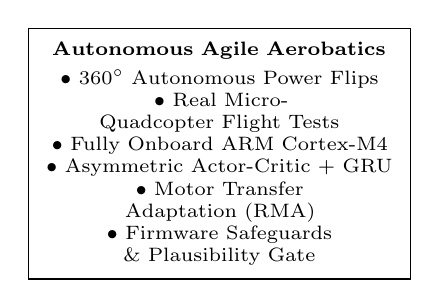
\begin{tikzpicture}
        \node[sblock, text width=4.5cm, inner sep=5pt] {
          \textbf{Autonomous Agile Aerobatics}\\[0.3em]
          \scriptsize
          $\bullet$ 360$^\circ$ Autonomous Power Flips\\
          $\bullet$ Real Micro-Quadcopter Flight Tests\\
          $\bullet$ Fully Onboard ARM Cortex-M4\\
          $\bullet$ Asymmetric Actor-Critic + GRU\\
          $\bullet$ Motor Transfer Adaptation (RMA)\\
          $\bullet$ Firmware Safeguards \& Plausibility Gate
        };
      \end{tikzpicture}
      
      \vspace{1.0em}
      {\footnotesize\bfseries Andreas Panagopoulos}\\[0.15em]
      {\scriptsize Department of ECE, University of Patras}\\[0.15em]
      {\scriptsize\texttt{andreas.panagopoulos@ac.upatras.gr}}\\[0.4em]
      {\scriptsize Open-Source: \texttt{github.com/andrupe/Quadcopter-flip}}
    \end{column}
  \end{columns}
\end{frame}

\end{document}
